\documentclass[compress]{beamer}
\usepackage[utf8]{inputenc}
\usepackage[francais]{babel}
\usepackage[T1]{fontenc}
\usepackage{amssymb}
\usepackage{amsmath}
\usepackage{amsfonts}
\usepackage{hyperref}
\usepackage[]{algorithm2e}
\usepackage{amssymb}
\usepackage{verbatim}
\usepackage{listings}
\usepackage{color}
\usepackage{graphicx}
\usetheme[navigation]{UMONS}

\author{Clément Tamines, Florent Delgrange}
\title{Temps, Horloge et l'ordonnancement de évènements dans un système distribué}

\setbeamercovered{transparent} 
\setbeamertemplate{navigation symbols}{} 
\institute{UMONS\\Faculté des Sciences\\MA1 Sciences Informatiques\\[2ex]
  
\includegraphics[height=4ex]{UMONS}\hspace{2em}%
  \raisebox{-1ex}{
\includegraphics[height=6ex]{UMONS_FS}}}
\date{novembre 2016} 
\definecolor{darkgreen}{rgb}{0.0, 0.2, 0.13}
\subject{Réseaux II} 

\begin{document}

\begin{frame}
\titlepage
\end{frame}

\begin{frame}
\tableofcontents
\end{frame}

\section{Introduction}

\begin{frame}
\begin{itemize}
\item Comment classer chronologiquement les évènements dans un système distribué ?
\item Comment définir le fait qu'un évènement A s'est passé avant un autre évènement B ?
\end{itemize}
\end{frame}

\begin{frame}
\frametitle{Système distribué}
	\begin{definition}
		Un système distribué est une collection de processus distincts qui sont séparés dans l'espace et qui communiquent entre eux par 			messages.
	\end{definition}
	Exemples : 
	\begin{itemize}
		\item Système de PC inter-connectés à l'aide d'un réseau de communication
		\item Un simple PC dans lequel l'unité de contrôle , les unités de mémoire et les canaux d'entrées/sorties sont des processus séparés.
		\item etc
	\end{itemize}
\end{frame}

\begin{frame}
\frametitle{Temps et ordonnancement ?}
Soient a et b, deux évènements. On dit que\\
\textit{a est arrivé avant b} si $a$ est arrivé plus tôt dans le temps que $b$.\\
\textbf{Horloge réelle : }n'est pas forcément exacte et ne fournit pas le temps au sens physique précis ! \\ $\implies$ la relation \textit{est arrivé avant} doit s'exprimer sans horloge réelle.\\
\end{frame}

\section{Ordre partiel}

\begin{frame}
\frametitle{\'Evènements}
Le système est composé d'une collection de processus et chaque processus est une séquence d'évènements.\\
exemple : L'exécution d'un sous-programme ou d'une instruction sur un ordinateur peut être considéré comme un évènement.\\
Les évènements d'un processus forment une séquence où a apparait avant b ssi a est exécuté avant b.
\begin{figure}
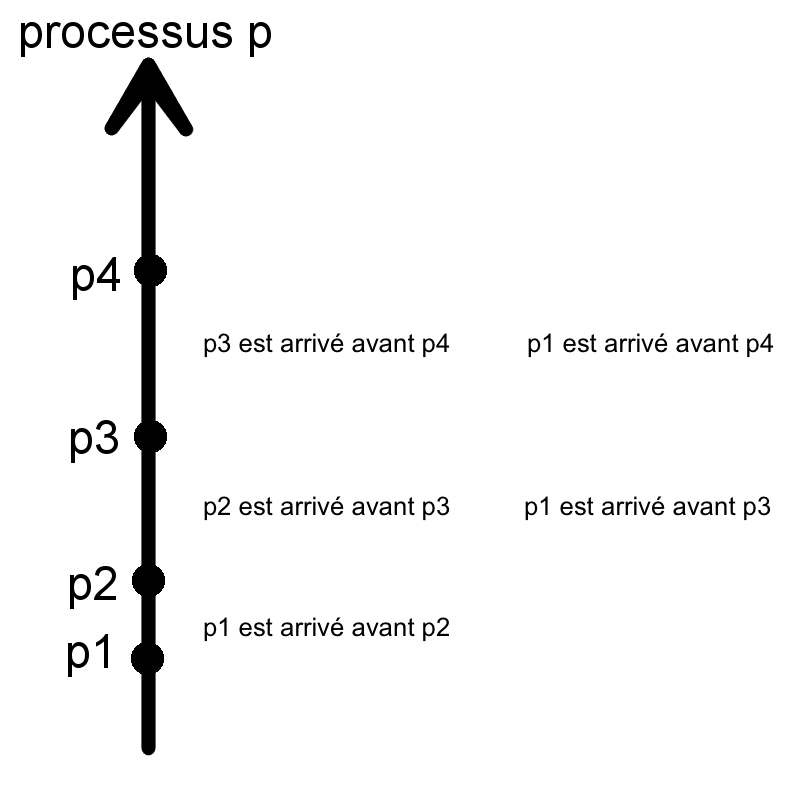
\includegraphics[scale=0.15]{process1.png}
\end{figure}
\end{frame}
\begin{frame}
On considère que envoyer/recevoir un message comme un évènement d'un processus.
\begin{definition}
La relation $\rightarrow$ sur un ensemble d'évènements d'un système satisfait
\begin{enumerate}
\item Si $a$ et $b$ sont des évènements du même processus et a vient avant b, alors $a \rightarrow b$.
\item Si $a$ correspond à l'envoi d'un message par un processus et b correspond à la réception de ce message par un autre processus, alors $a \rightarrow b$.
\item $\rightarrow$ est transitif. On dit que 2 évènements $a, b$ sont concurrents ssi $a \not\rightarrow b$ et $b \not\rightarrow a$
\end{enumerate}
\end{definition}
\end{frame}

\begin{frame}
\begin{figure}
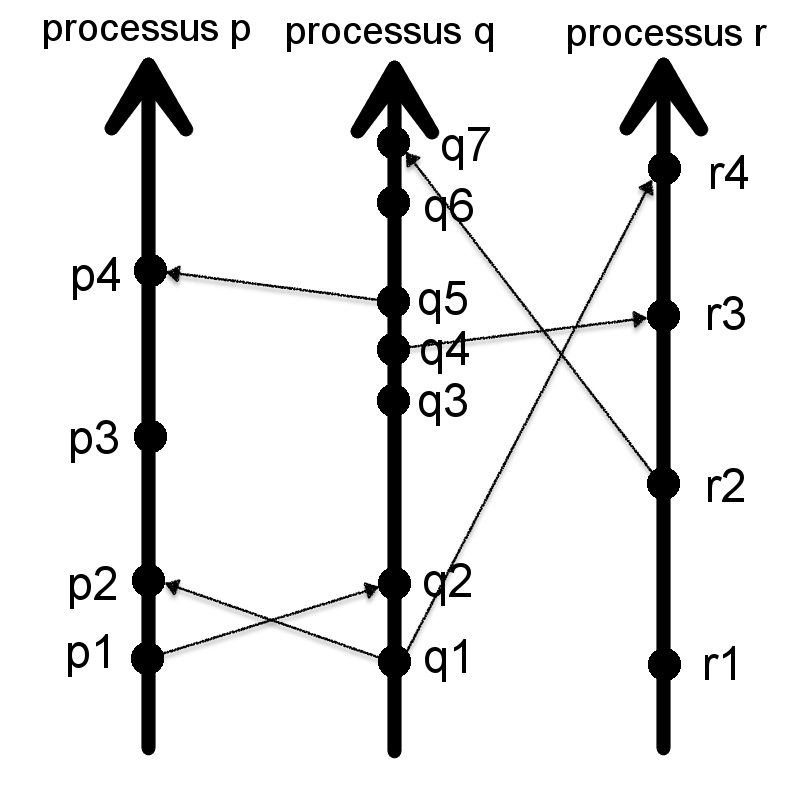
\includegraphics[scale=0.3]{process2.png}
\end{figure}
\end{frame}

\begin{frame}
  \begin{columns}
    \begin{column}{.5\textwidth}
    \begin{block}{}
		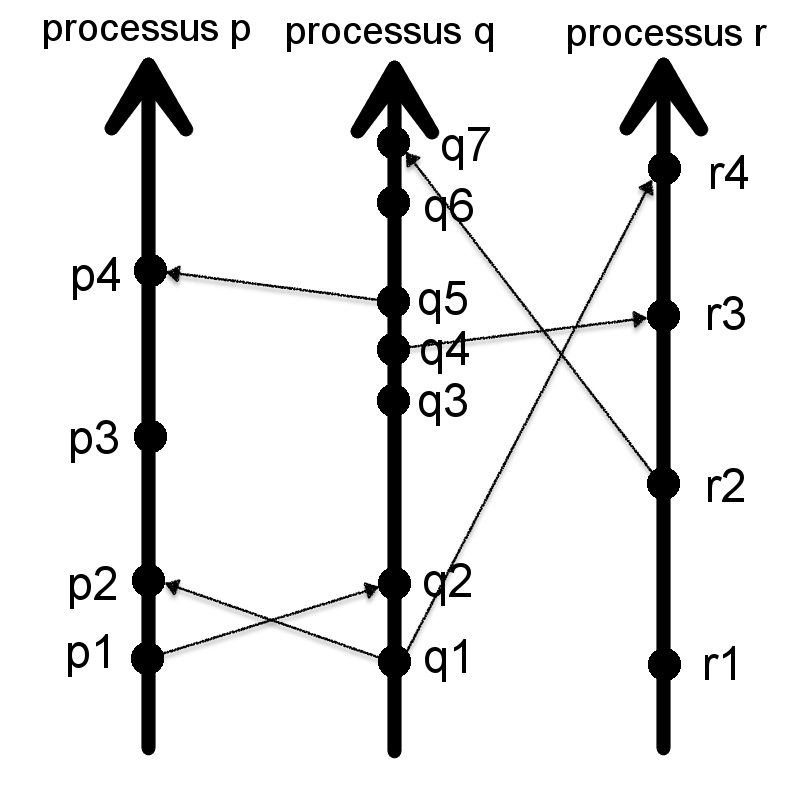
\includegraphics[scale=0.15]{process2.png}
    \end{block}
    \end{column}
	\begin{column}{0.5 \textwidth}
	\begin{block}{}
		$a \rightarrow b$ signifie que $a$ peut aller vers $b$ sur le diagramme en avançant dans le temps le long du processus et de la ligne de message.
		\end{block}
	\end{column}
	\end{columns}
	Par exemple on a $p_1 \rightarrow r_4$  par transitivité avec \\
	$p_1 \rightarrow q_2$ et $q_2 \rightarrow q_3$ et $q_3 \rightarrow q_4$ et $q_4 \rightarrow r_3$ et $r_3 \rightarrow r_4$\\
	\textbf{{\color{red}Problème : }}on voit par exemple que $q_3$ est concurrent avec $p3$ ; on ne sait pas si $q_3$ s'est passé avant $p_3$ et vice versa.
\end{frame}

\section{Horloges Logiques}

\begin{frame}
\frametitle{Horloges logiques}
Une horloge est juste une façon d'assigner un numéro à un évènement où le numéro correspond au temps où l'évènement s'est produit.\\
$\implies$ Chaque processus $p_i$ est associé à une horloge $C_i$.\\
$\implies$ Pour tout évènement $a$ se produisant dans $P_i$, on assigne un nombre $C_i$<$a$> \\
Le système entier est donc représenté par la fonction $C$.\\
\begin{block}{Propriétés}
\begin{itemize}
\item Soit b, un évènement, $C$<$b$>$ = C_j$<$b$> ssi $b$ est un évènement du processus $P_j$.\\
\item $\forall i$, $C_i$ peut être simplement implémenté à l'aide de compteurs sans mécanisme lié au temps.
\end{itemize} 
\end{block}
\end{frame}

\begin{frame}
\frametitle{Conditions}
\begin{block}{Condition faible}
$a \rightarrow b \implies C$<$a$> $ < C$<$b$>
\end{block}
Cela implique que 2 évènements concurrents doivent se produire en même temps. Sur la figure, on a que $p_2$ et $p_3$ sont concurrents de $q_3$. Donc on devrait avoir que $p_2 = p_3 = q_3$ et cela contredit le fait que $p_2 < p_3$.
\begin{block}{Conditions fortes}
\begin{enumerate}
\item Si $a$ et $b$ sont des évènements de $P_i$ et que $a$ vient avant $b$, alors $C_i$<$a$> $<$ $C_i$<$b$>
\item Si $a$ est l'envoi d'un message par un processus $P_i$ et que $b$ est la réception de ce message par le processus $j$, alors $C_i$<$a$> $< C_j$<$b$>
\end{enumerate}
\end{block}
\end{frame}

%\begin{frame}
%\begin{figure}
%		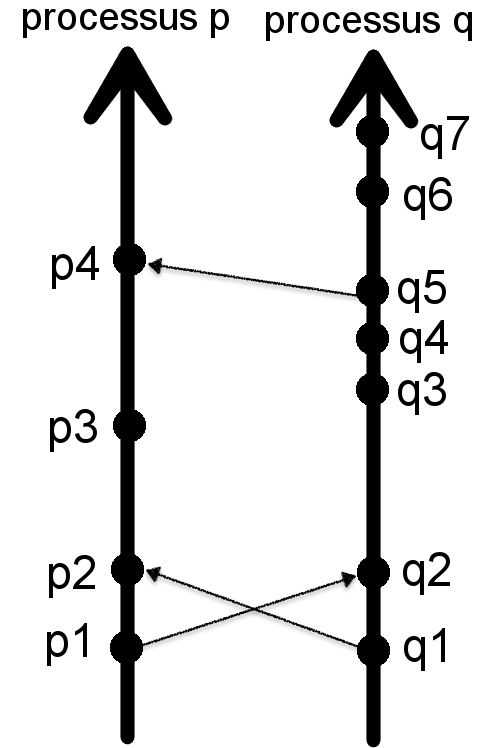
\includegraphics[scale=0.17]{process3.png}

%\end{figure}
%\textbf{Exemples : }\\
%		$C$<$p_1$> $< C$<$p_3$>\\
%		$C$<$q_5$> $< C$<$p_4$>
%\end{frame}

\begin{frame}
\frametitle{Implémentation}
On veut garantir que la {\color{cyan} condition 1} soit respectée. Il suffit que $C_i$ se plie à la règle d'implémentation suivante : 
\begin{block}{IR 1}
Chaque processus $P_i$ incrémente $C_i$ entre 2 évènements successifs.\\
Soient $a$, $b$, deux évènements successifs de $P_i$. Alors, $C_i \leftarrow C_i + 1$.
\end{block}
\end{frame}

\begin{frame}
	\frametitle{Implémentation}
	Pour garantir la {\color{cyan} condition 2}, il faut que chaque message $m$ contienne un TimeStamp $T_m$ qui est égal au temps $t$ où le message a été émis. \\
	\textbf{But : }Lorsqu'un message $m$ est reçu, un processus avance son horloge de telle sorte à ce que celle-ci soit $>$ à $T_m$
	\begin{block}{IR 2}
	\begin{enumerate}[(a)]
		\item Si un évènement $a$ est l'envoi d'un message $m$ par le processus $P_i$, alors le message $m$ contient un Timestamp $T_m \leftarrow C_i$<$a$>
		\item Lorsqu'il reçoit un message $m$, le processus $P_j$ met à jour la variable $C_j$ tel que $C_j > T_m$ et $C_j \geq$ valeur courante de $C_j$
	\end{enumerate}
	\end{block}
\end{frame}

\section{\'Evènements totalement ordonnés}
\begin{frame}
\frametitle{Ordre total}
On souhaite avoir un système d'horloge qui satisfait les conditions d'horloge précédemment énoncées et qui met en place un \textit{\textbf{ordre total}}.\\
\textbf{Rappel : }
\begin{block}{Ordre Total}
Une \textbf{relation binaire} $\preceq$ sur un ensemble E est un ordre total si $\forall x, y, z \in E$, \\
\begin{itemize}
\item \textbf{Réflexivité :} $x \preceq x$
\item \textbf{Antisymétrie :} $x \preceq y$ et $y \preceq x \implies x = y$
\item \textbf{Transitivité :} $x \preceq y$ et $y \preceq z \implies x \preceq z$
\end{itemize}
\end{block}
\end{frame}

\begin{frame}
\frametitle{Ordre Total}
Soit $\preceq$, un ordre total arbitraire. On définit une relation $\implies$ comme suit :\\
Si $a \in P_i$ et $b \in P_j$, alors \\
\[
	a \Rightarrow b \ \ \text{ssi}
	\begin{cases}
		C_i \text{<}a\text{>} < C_j\text{<}b\text{>} \\
		\text{ou}\\
		C_i\text{<}a\text{>} = C_j\text{<}b\text{>} \text{ et } P_i \prec P_j
	\end{cases}
\]
\end{frame}

\end{document}